%%%%%%%%%%%%%%%%%%%%%%%%%%%%%%%%%%%%%%%%%
% Original author:
% Linux and Unix Users Group at Virginia Tech Wiki 
% (https://vtluug.org/wiki/Example_LaTeX_chem_lab_report)
%
% License:
% CC BY-NC-SA 3.0 (http://creativecommons.org/licenses/by-nc-sa/3.0/)
%
%%%%%%%%%%%%%%%%%%%%%%%%%%%%%%%%%%%%%%%%%

%----------------------------------------------------------------------------------------
%	PACKAGES AND DOCUMENT CONFIGURATIONS
%----------------------------------------------------------------------------------------

\documentclass[a4paper,11pt]{article}

\usepackage{graphicx} % Required for the inclusion of images
\usepackage{titling}
\usepackage{upgreek}

\setlength{\droptitle}{-8em}   % This is your set screw

\setlength\parindent{0em} % Removes all indentation from paragraphs

\renewcommand{\labelenumi}{\alph{enumi}.} % Make numbering in the enumerate environment by letter rather than number (e.g. section 6)

\usepackage{times} % Uncomment to use the Times New Roman font

%\usepackage{indentfirst}

\setlength{\parskip}{0.5em plus1pt minus1pt}

%\usepackage{showframe} % for viewing margin frames (debug)

% \usepackage{fullpage}

\usepackage{hyperref}

%----------------------------------------------------------------------------------------
%	DOCUMENT INFORMATION
%----------------------------------------------------------------------------------------

\title{SDP Group 8: Final Group Report} % Title

% \author{Blake Hawkins} % Author name

\date{21 April, 2014} % Date of the milestone

\begin{document}

\maketitle % Insert the title, author and date

\begin{center}
\textbf{Mentor:} Katharina Heil, \textbf{Guest Mentor:} Tom Spink % Instructor/supervisor
\\
\textbf{Members:} Blake Hawkins, % Partner names
Lubomir Vikev,
Borislav Ikonomov,
Yordan Stoyanov,
James Linehan,
Lukas Dirzys,
Iain Brown,
Emanuel Martinov,
Robaidh Mackinnon,
Aneesh Ghosh

\end{center}

%----------------------------------------------------------------------------------------
%   SECTION 1 (Introduction)
%----------------------------------------------------------------------------------------

\section{Introduction}

Our goal for the course was to produce a reliable, extensible set of code to control a pair of robots during a football match, with the potential to win the final tournament. We achieved consistent top-2 performance in milestones and friendly matches, and placed third in the final tournament. 

This report aims to describe the steps we took regarding all aspects of the project to achieve these goals. It is divided up into loosely separable sections, each of which will mention the tasks we faced, solutions we deployed, problems we endured, lessons we learned, and our achievements. 



%----------------------------------------------------------------------------------------
%	SECTION 2 (Management and Organisation)
%----------------------------------------------------------------------------------------

\section{Management and Organisation}

Our first day of SDP began with a group discussion of how to go about managing our team; we agreed that having a remote repository, issue tracker, and facebook group were invaluable. Without specific intervention, the majority of our group arrived daily and were actively involved with resolving various issues. This naturally progressed into daily informal group work, similar to a scrum.

As the semester progressed our issue tracker also became a centralised source of tutorials and event calendaring, in the form of a wiki. Along with paired programming and code review, things started smoothly and only improved as milestones were met. By the time of the first assessed friendly match, it was apparent to us that we were doing many things right.

Now that the final tournament has ended, we are left with some time to consider our process more theoretically. We wonder how things would have run differently with an official project manager, and compare ourselves to other groups. Using github's internal issue tracker and wiki  server may have saved us time, but would not have any major effect. For an academic group effort, our free-for-all environment was likely difficult to deal with for some students, and a more traditional management scheme may have improved that.



%----------------------------------------------------------------------------------------
%	SECTION 3 (Hardware)
%----------------------------------------------------------------------------------------

\section{Hardware}

In terms of robotics, our goal was to demonstrate a design with the features necessary to quickly and reliably navigate a pitch region, manipulate a ball, score goals, and pass to a partner. We were pleased with our final product, but not without significant changes throughout the semester.

Our group used Lego Mindstorms hardware running the LejOS firmware and NXJ JVM  on the NXT “Intelligent Brick”. We chose to use a 4-wheel-drive chassis, a stable design with efficient use of torque and high maximum speed, using LejOS’ differential controller methods. Rubber tyres in this design caused the robot to stutter and jump when turning in place. Our solution was to use tyreless wheels to reduce friction. Holonomic wheels were another potential design tool, but we decided their lack of guarantee in effectiveness combined with high price was a gamble we were not willing to take.

During roughly the first half of the project, our group had substantial difficulties in terms of the robots’ kicker strength - it was too weak for bounce shots, and sometimes failed even direct shots. Solving this issue was of high priority, so we experimented with many different designs to combat this particular problem. 

For Milestone \#2, which tested the robots' kicking ability, we attempted to use pneumatics - an external battery would constantly power a pump, which in turn would compress air inside a tank, later released to operate the kicker. This design was sufficiently powerful and completed the milestone efficiently, but had many drawbacks - the kicker strength was not easily controllable, time was needed to compress the air in the tank between matches, and the design also occasionally suffered from explosive failure. Although weaker, a mechanical kicker was much more dependable and therefore our final choice.

After working on Milestone \#3, we decided a ball grabber would improve our ability to control and react to the ball. We initially explored the possibility to have the grabber and kicker use a single motor powered by the NXT Brick. However, the kicker was prohibitively weak due to the extra weight of the grabber that needed to be moved, and the loss of torque through to the additional gearing.

As a result, we added an I2C Motor Multiplexer to extend the motor limit, allowing the use of 9v motors to operate the grabber. This freed an NXT motor slot to be used entirely for the servo-operated kicker, which was driven by a spring-tensioned chain to prevent gear slipping.



%----------------------------------------------------------------------------------------
%	SECTION 4 (Communications)
%----------------------------------------------------------------------------------------

\section{Communications}

Efficient and fast transmission of data between our systems was important for the correct and timely performance of our robots. After an initial discussion we agreed that the connection to the robots should run in a separate application. This allowed us to maintain a constant connection to both robots, and thereby improve the rate at which we could test iterations of strategy code.

Communication were handled in two stages: we used a TCP connection to send calculated commands from our strategy system to our command relay, which in turn sent data to the NXT Brick via bluetooth.

Initially, our communications client supported one robot per instance, and each command was sent as a pair of packets - a char that represented the command, and an integer that indicated power. This resulted in too much overhead, which severely limited our maximum command rate. After many incremental improvements, we arrived at the final version - one multithreaded application with a GUI which allowed us to easily connect/disconnect either robot and assign them arbitrarily as an attacker/defender. More importantly, each command would now be a single packet consisting of bytecode - this solved the problem with the overhead, and achieved a transmission time of about 1ms per command.

%----------------------------------------------------------------------------------------
%	SECTION 5 (Vision and World State)
%----------------------------------------------------------------------------------------

\section{Vision and World State}

The vision system was to use the overhead camera feed to reliably track the positions of the ball and robots, as well as the robots' orientations. This proved to be a difficult task due to changing illumination, large amounts of noise, similar colours, and subtle differences in camera optics and feed quality. In the end, we handled these issues to a reasonable extent, but our system still faces a few challenges.

Our vision code was initially based on Team 1's from 2013 since it was relatively easy to understand. However, for improved software design, and due to the new rules and goals this year, we made major refactorings and changes to improve modularity and expandability. We used the V4J4L library, and also experimented with OpenCV, which crashed the JVM due to outdated drivers; and OpenGL, which introduced a prohibitive amount of delay without a shared memory bus.

We were initially using a previous team's GUI code but later rewrote it from scratch using WindowBuilder. This allowed us to not only choose appropriate color thresholds for different objects (e.g. the ball, the yellow colour patch, etc.) but to also easily extend and modify the interface as requirements changed. With this manual calibration, our vision could be adjusted to high levels of precision when needed. Adjusting this system often took significant time, so we later added an option to simply click on a pixel to automatically adjust an object's thresholds to be near that pixel's values. This method was slightly less precise, but it saved a lot of time during testing.

At first, the system simply checked every pixel in the image and compared its values to the thresholds. This worked well for the ball, the green plates, and to an extent the yellow team's colour patch. However, there were significant problems with the blue team's patch and the black dots that were used for orientation - both had other pixels on the pitch that had very similar RGB and HSV values. Our solution was to first detect the green plates using K-means clustering, and then search for blue/yellow/black pixels only within the plates. This noticeably improved robot position and orientation tracking. To further improve the frame-rate we first constricted the processed area to a rectangle and later implemented an automatic pitch detection algorithm to further reduce this area. This, in combination with concurrent processing of the parts deemed important gave us near-optimal FPS. 

We used several methods to handle noise and distortion in order to get a more accurate picture of the playing field. We used a median filter to remove noise that would skew our results and greatly helped us in detecting plates. We also filtered object positions using small Gaussians to remove any remaining noise. Another filter we added, due to the ball-grabbing requiring exceptionally high precision to work properly, was to correct the fisheye distortion caused by the camera lens, which noticeably improved the accuracy of the data. To further improve this aspect, we removed the parallax displacement by using an algorithm that would project the robot plate positions down to the level of the pitch floor.
    

%----------------------------------------------------------------------------------------
%	SECTION 6 (Strategy)
%----------------------------------------------------------------------------------------

\section{Strategy}

We needed a strategy system that could cope with complex directions, be easily interruptible, deal with temporarily incorrect commands, follow the rules, and solve challenges rapidly.

Our implementation uses a non-blocking, asynchronous design: a pattern which depends on constant, correcting commands which solve a problem based on observation and reaction. The robot decision model was organised into a map of states based on ball position and speed, and any more complex strategies, such as bounce-passing or trying to trick the opposing defender, would be built using sub-states. Our final iteration featured multiple passing and scoring strategies, and was able to deal with all opponents faced.

Our final system has a total, cumulative delay of about 0.5 seconds, which made defending against goals difficult to deal with. We are confident that with more time we could improve our latency by making iterative changes to processing bottlenecks.

One other important observation is that the leJOS subsumption architecture provides a potential alternative to our naive decision model implementation that could improve performance and expandability. Whether using it would have improved our final performance, however, is difficult to say with any certainty without testing it.



%----------------------------------------------------------------------------------------
%	SECTION 7 (Conclusion)
%----------------------------------------------------------------------------------------

\section{Conclusion}

In general, we are pleased with our performance - the team worked well together as a group, as was reflected in the results achieved throughout the semester. We received high marks in the milestones and assessed friendly matches (21 of a possible 24 marks). As the result of our performance we placed third in the final tournament.

If we were to repeat the process, we could potentially improve the organisation of the team both in development and planning thereof. We would occasionally have multiple people working on the same problem without communicating with each other, which could be addressed.

One interesting point is that our group spent £0 of our allocated finances, so considering useful parts for purchase is one improvement point. We had considered using a holonomic-wheeled robot chassis design, but discounted it on the basis of much more complicated movement and tactical coding to fully utilise the capabilities of such a chassis. Had we been given more time to work on the project, it was felt that such a design would be feasible and may well improve our performance in matches.
    
    
    
%----------------------------------------------------------------------------------------
%	SECTION 8 (Appendices)
%----------------------------------------------------------------------------------------

\section{Appendices}

Below are some links and screenshots to aid in the reader's understanding of our group's works and tools used for work management and organisation. 

\subsection{Links to our Resources}

\begin{itemize}
	\item \url{http://www.github.com/vikev/SDP} - Git Repository
	\item \url{http://trac.no-ip.biz/} - Bug Tracker and Wiki; Note, this is hosted on a personal web server and may be temporarily unavailable
\end{itemize}

\subsection{Figures}

\begin{figure}[p]
    \centering
    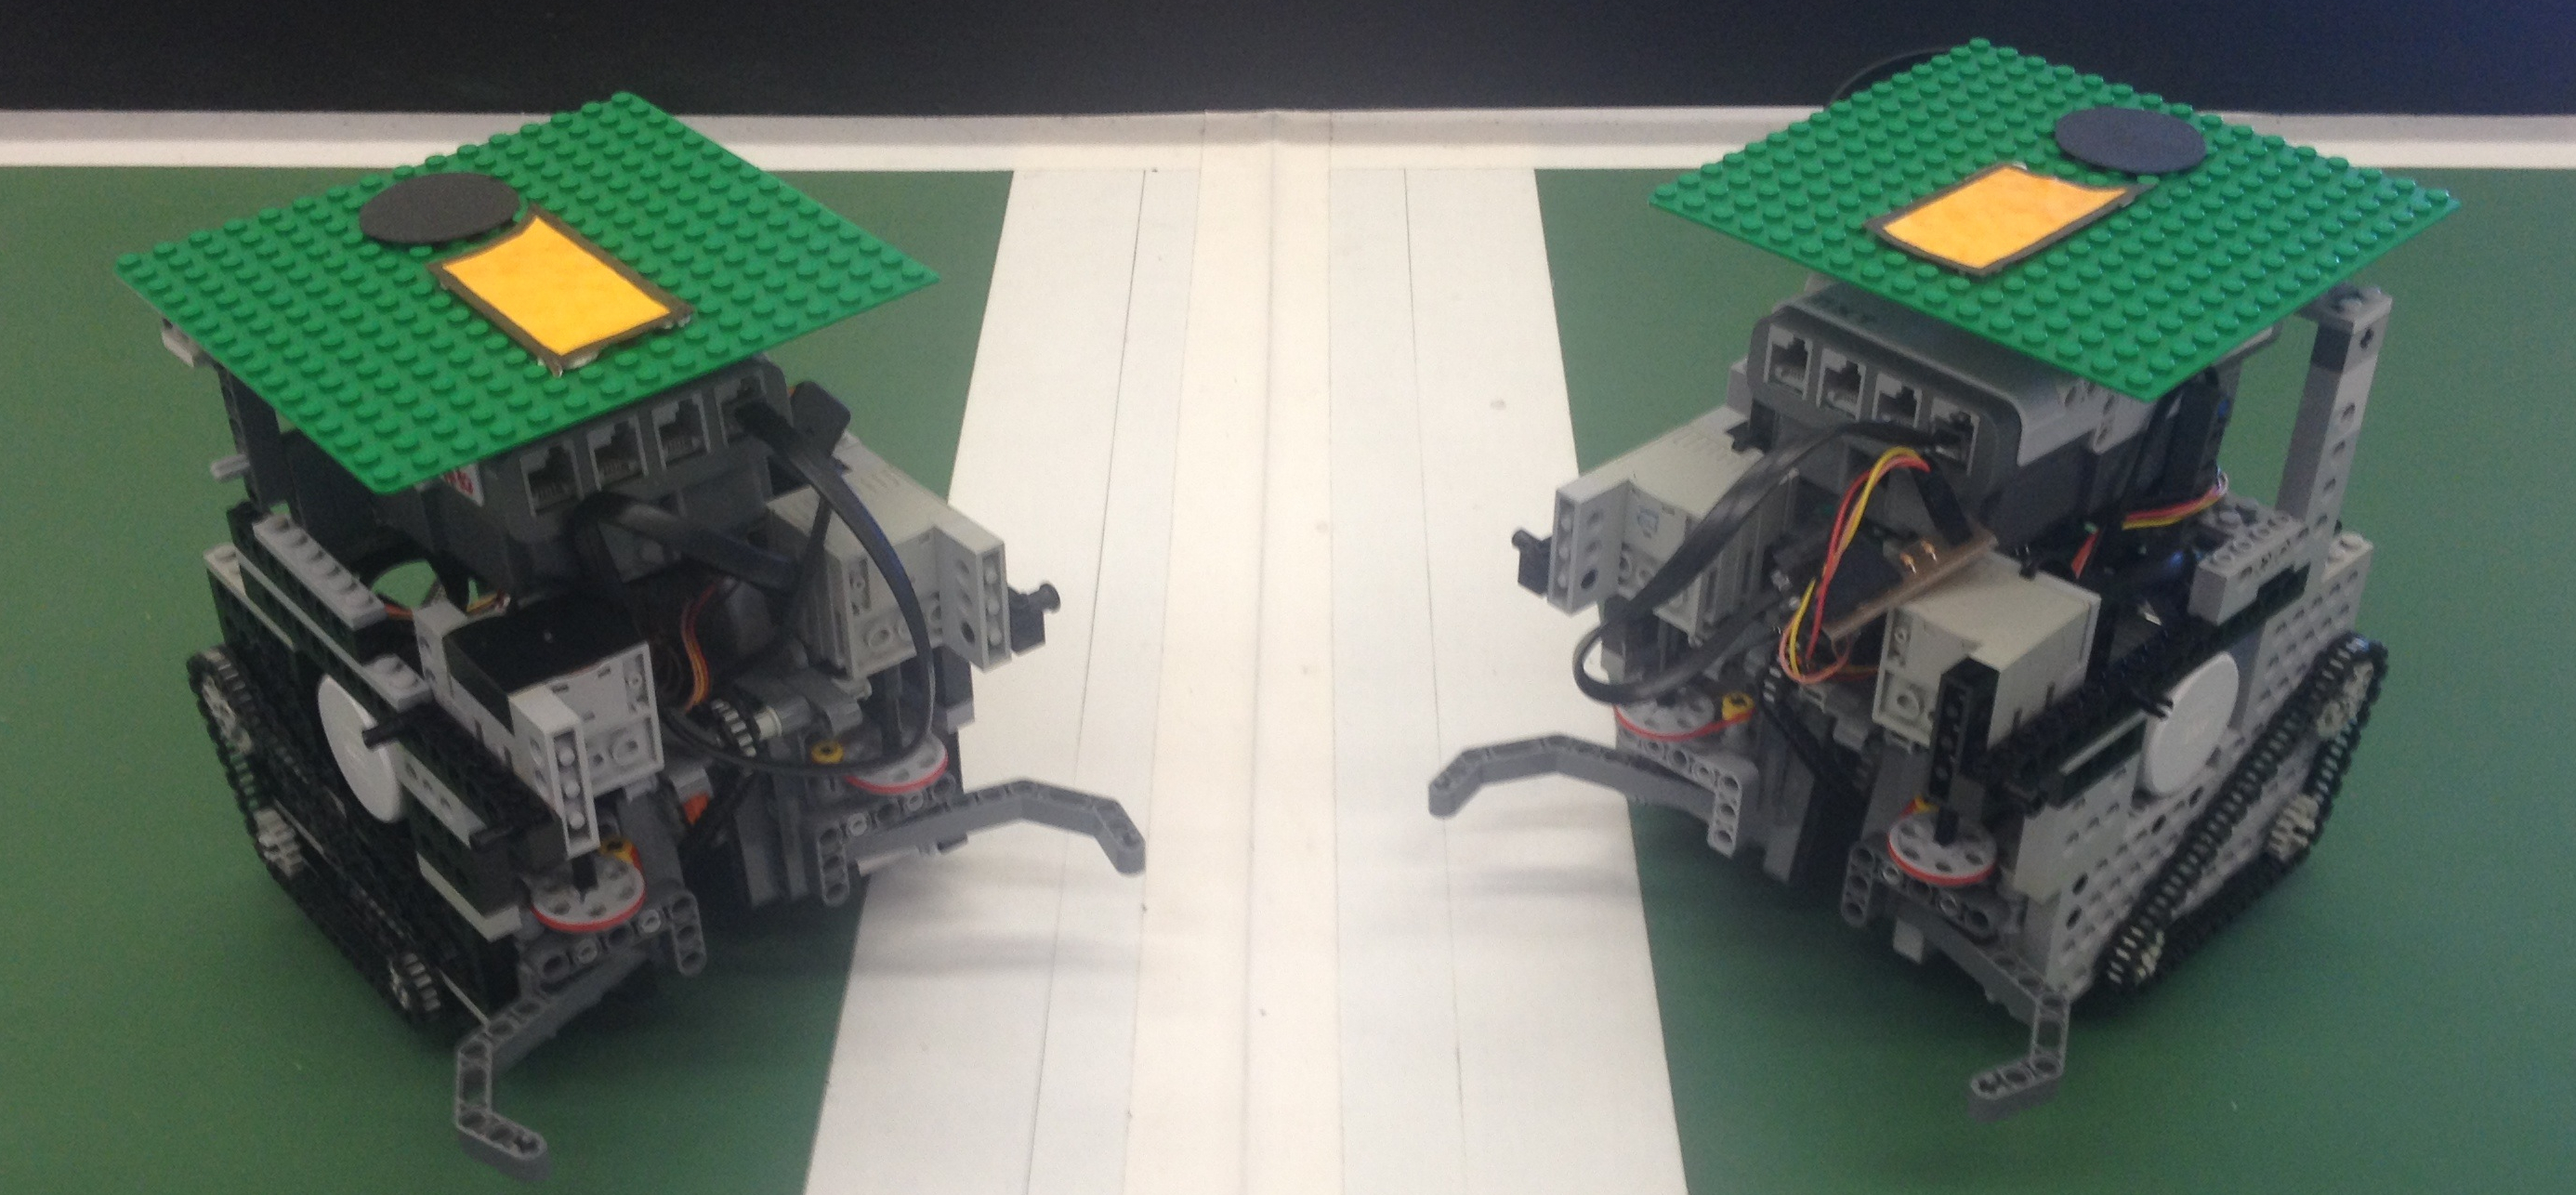
\includegraphics[width=130mm]{both_robots_cropped.jpg}
    \caption{Two Identical Robots}
\end{figure}

\begin{figure}[p]
    \centering
    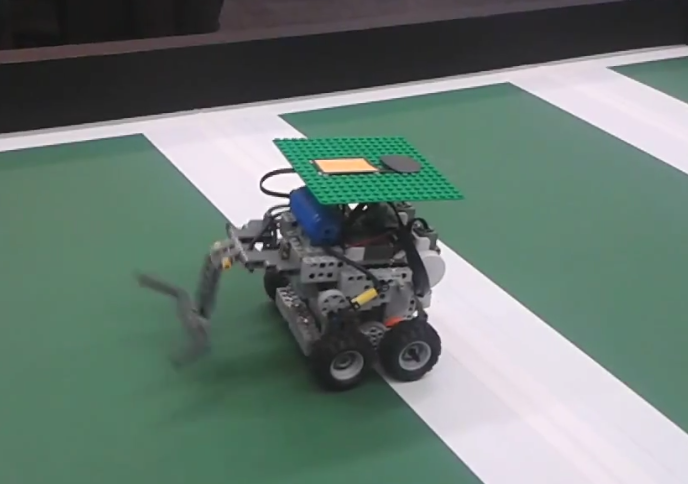
\includegraphics[width=110mm]{pneumatic.png}
    \caption{Pneumatic Kicker Design}
\end{figure}

\begin{figure}[p]
    \centering
    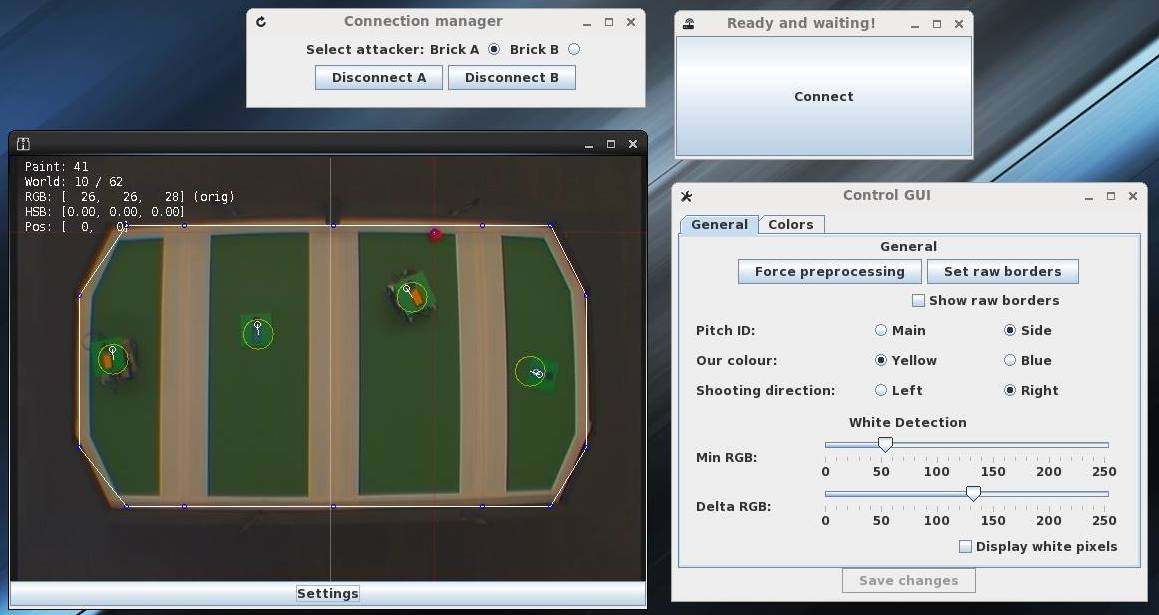
\includegraphics[width=110mm]{system.jpg}
    \caption{Our System GUI}
\end{figure}

\begin{figure}[p]
    \centering
    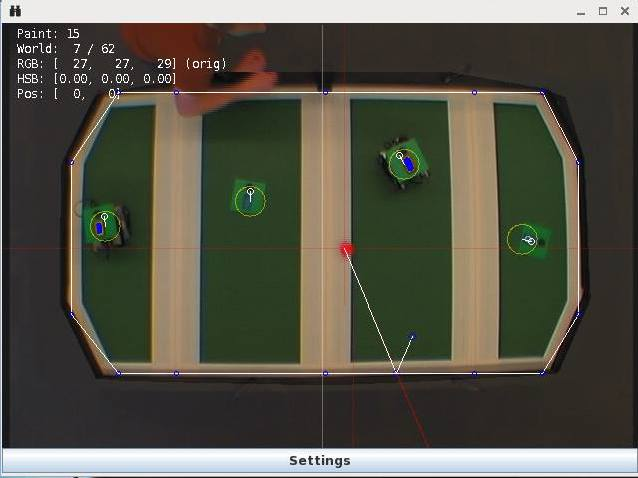
\includegraphics[width=110mm]{system2.jpg}
    \caption{Ball Prediction}
\end{figure}

\begin{figure}[p]
    \centering
    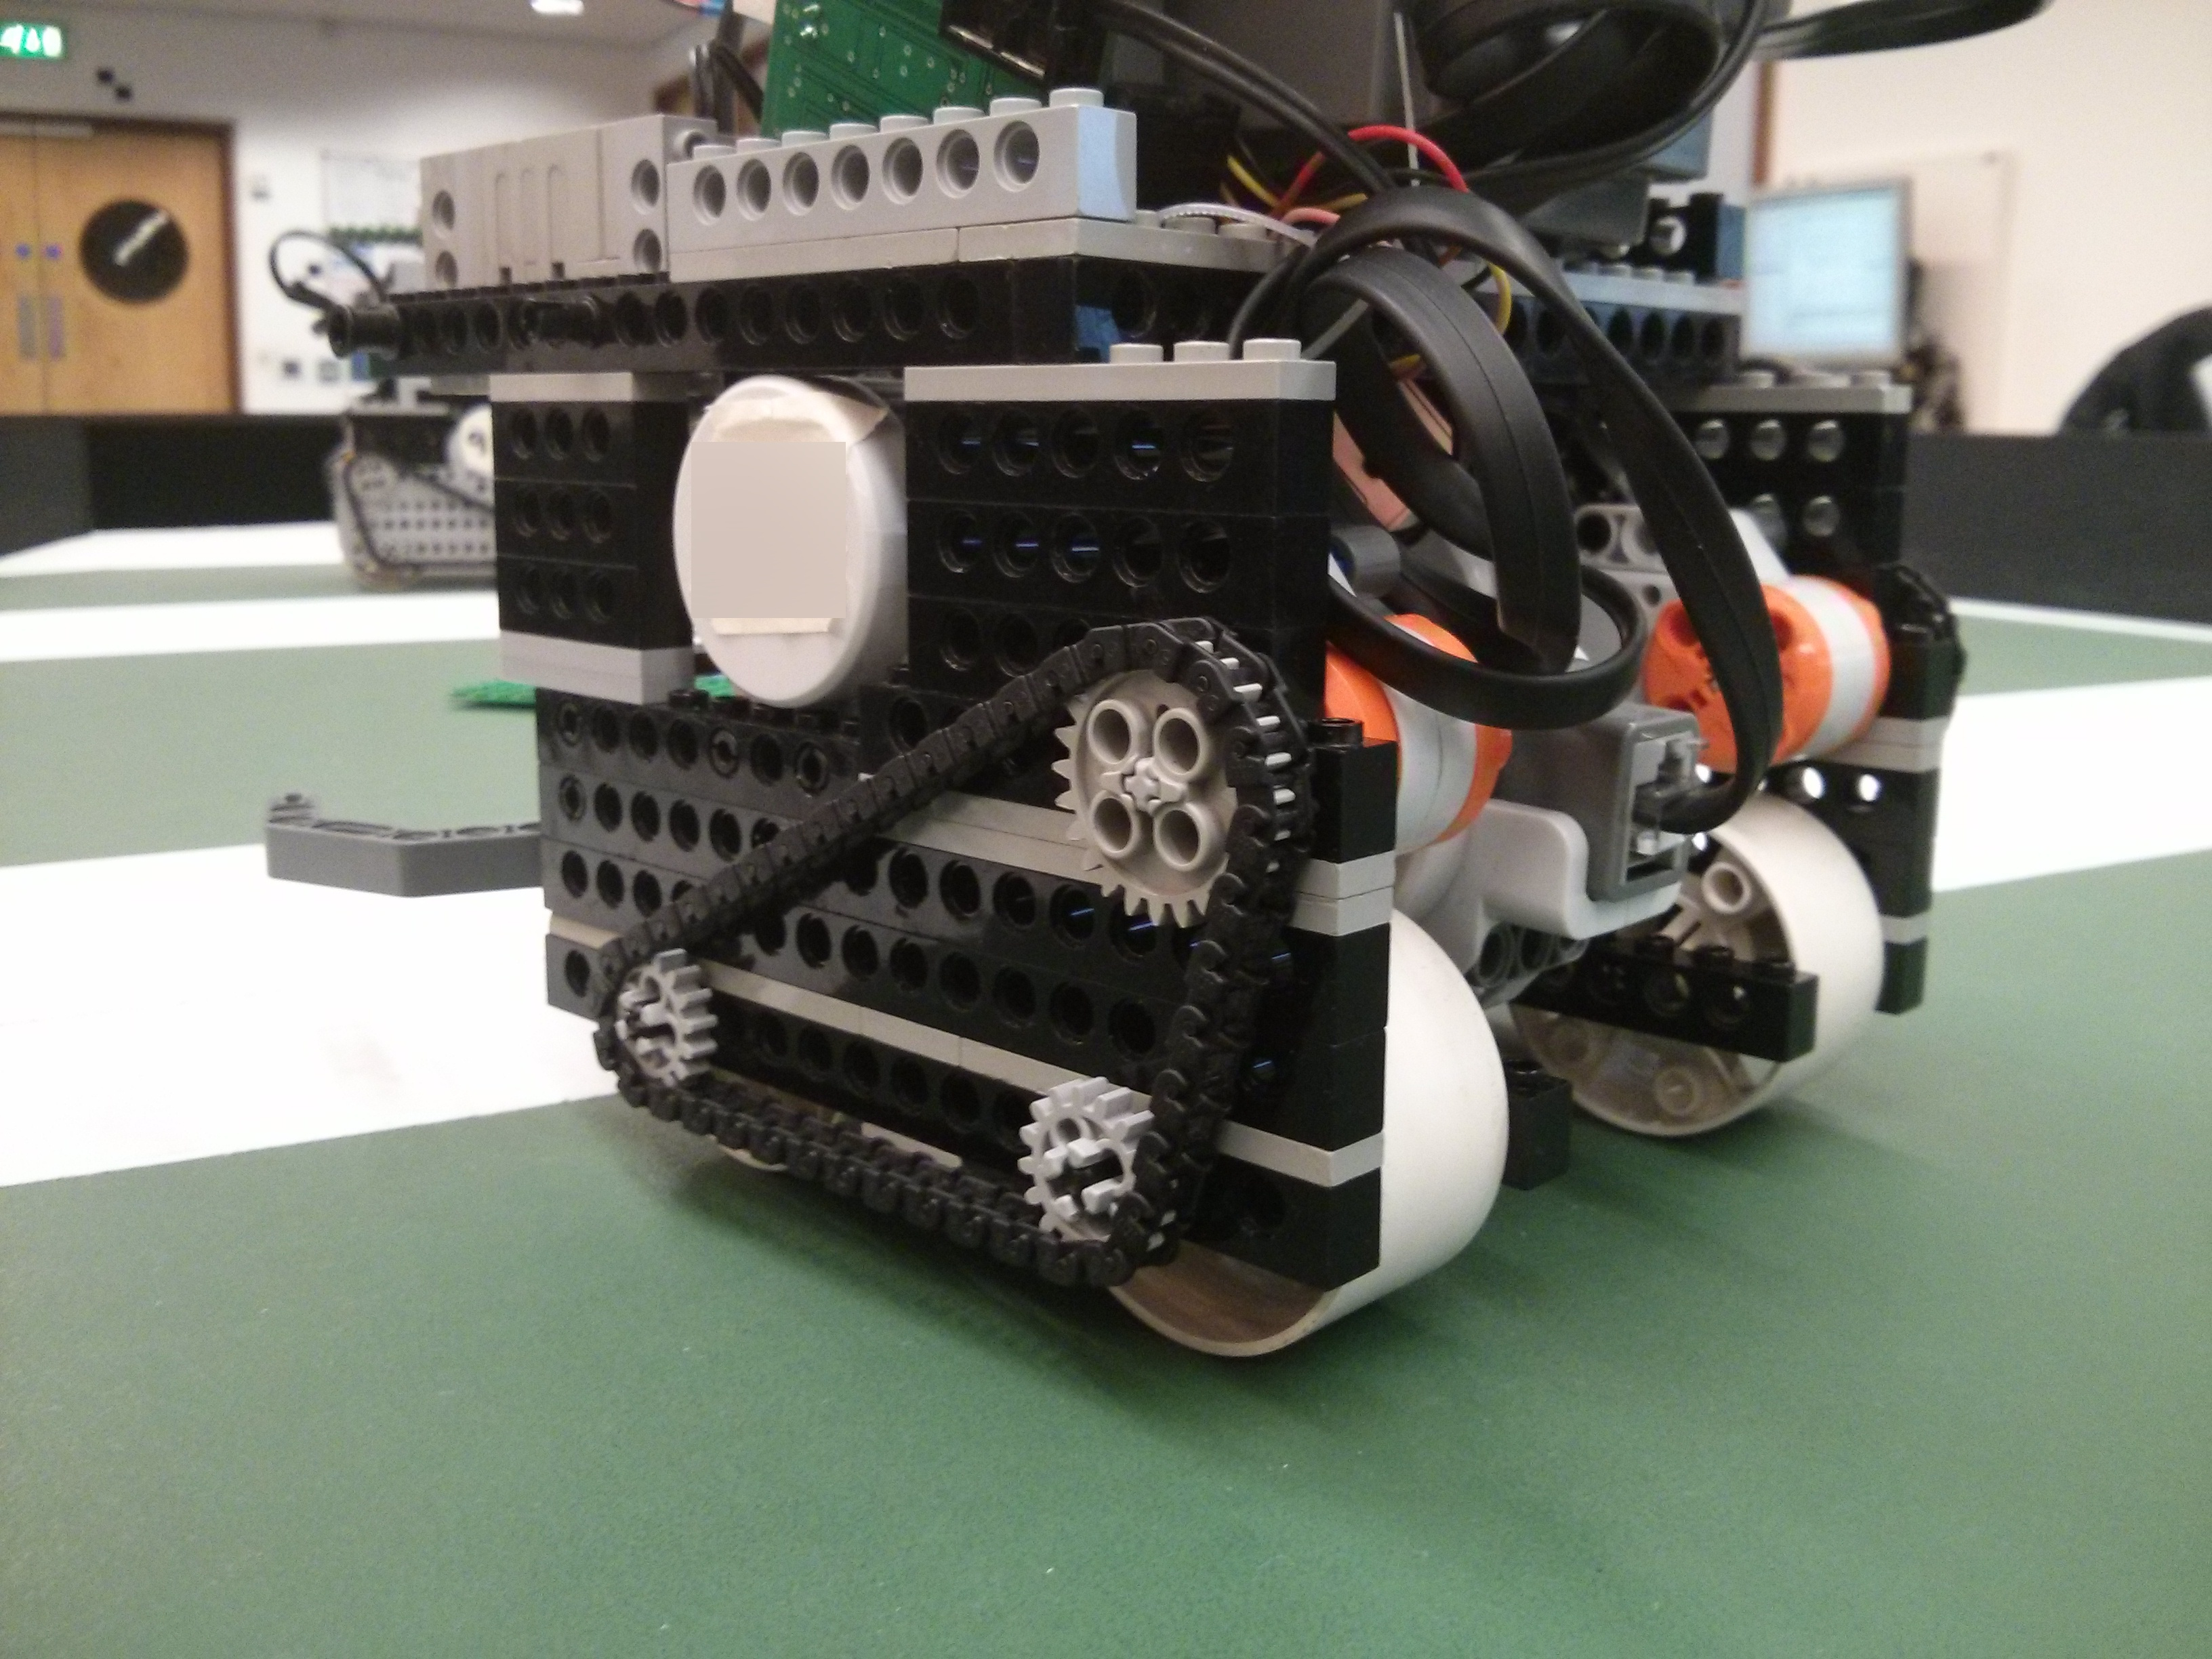
\includegraphics[width=130mm]{wheels-image.jpg}
    \caption{Tyreless Wheels}
\end{figure}

\end{document}



